\documentclass[%
%reprint,
%superscriptaddress,
%groupedaddress,
%unsortedaddress,
%runinaddress,
%frontmatterverbose, 
%preprint,
%preprintnumbers,
%notitlepage,
%nofootinbib,
%nobibnotes,
%bibnotes,
 amsmath,amssymb,
aps,
 %prl,
%pra,
%prb,
%rmp,
%prstab,
%prstper,
%floatfix,
]{revtex4-2}

\usepackage{graphicx}% Include figure files
\usepackage{dcolumn}% Align table columns on decimal point
\usepackage{bm}% bold math
\usepackage{hhline}
%\usepackage{subfigure}
\usepackage{subcaption}
\usepackage{caption}
\usepackage{multirow}
\usepackage{booktabs}
\usepackage{xr}
\usepackage[dvipsnames]{xcolor}
\usepackage{nicefrac}
\usepackage{etoolbox}
\patchcmd{\section}
  {\centering}
  {\raggedright}
  {}
  {}
\patchcmd{\subsection}
  {\centering}
  {\raggedright}
  {}
  {}
\graphicspath{{figs/}}
%hack to have outline that is not spaced so wide
\newcommand{\ItemSpacing}{0pt}%
\newcommand{\ParSpacing}{0pt}%
% \newcommand{\TODO}{{\color{Red}\textbf{TODO}}}%
\newcommand{\TODO}[1]{{\color{red}\textbf{TODO: }{#1}\normalcolor}} %TODO
\newcommand{\com}[1]{{\color{blue}[{#1}]\normalcolor}} %Comment
\newcommand{\brycerev}[1]{{\color{Purple}{#1}\normalcolor}} %Comment
\newcommand{\brycecom}[1]{{\color{ProcessBlue}[{#1}]\normalcolor}} %Comments from Bryce
\newcommand{\rosscom}[1]{{\color{Orange}[{#1}]\normalcolor}} %Comment from Jacob 
\newcommand{\kiercom}[1]{{\color{Green}[{#1}]\normalcolor}} %Comment from Kieran


\newcommand{\UpperState}{3^{3\!}S_1}%
\newcommand{\MetastableState}{2^{3\!}S_1}%
\newcommand{\MidState}{2^{3\!}P_{0,1,2}}%
\newcommand{\GroundState}{1^{1\!}S_{0}}%
\newcommand{\avg}[1]{\left\langle #1 \right\rangle}
% Outlines configurations
\usepackage{outlines}
\usepackage{enumitem}
\setenumerate[1]{itemsep={\ItemSpacing},parsep={\ParSpacing},label=\Roman*.}
\setenumerate[2]{itemsep={\ItemSpacing},parsep={\ParSpacing},label=\Alph*.}
\setenumerate[3]{itemsep={\ItemSpacing},parsep={\ParSpacing},label=\roman*.}
\setenumerate[4]{itemsep={\ItemSpacing},parsep={\ParSpacing},label=\alph*.}
\usepackage{hyperref}

\makeatletter
\newcommand*{\addFileDependency}[1]{% argument=file name and extension
  \typeout{(#1)}
  \@addtofilelist{#1}
  \IfFileExists{#1}{}{\typeout{No file #1.}}
}
\makeatother
 
\newcommand*{\myexternaldocument}[1]{%
    \externaldocument{#1}%
    \addFileDependency{#1.tex}%
    \addFileDependency{#1.aux}%
}

\myexternaldocument{main}

%\usepackage{hyperref}% add hypertext capabilities
%\usepackage[mathlines]{lineno}% Enable numbering of text and display math
%\linenumbers\relax % Commence numbering lines

%\usepackage[showframe,%Uncomment any one of the following lines to test 
%%scale=0.7, marginratio={1:1, 2:3}, ignoreall,% default settings
%%text={7in,10in},centering,
%%margin=1.5in,
%%total={6.5in,8.75in}, top=1.2in, left=0.9in, includefoot,
%%height=10in,a5paper,hmargin={3cm,0.8in},
%]{geometry}
\renewcommand\thefigure{S\arabic{figure}}
\renewcommand{\thetable}{S\arabic{table}} 
\begin{document}
\title{Supporting Online Material}
%\appendix
\maketitle

\section{Experimental Details}
\label{sec:exp-details}
\begin{figure}
    \centering
    \includegraphics[width=0.6\textwidth]{SOMs/beam_waist.png}
    \caption{Beam diameter (twice the beam width \(w\)) of the probe beam over relative distance along the axis of the probe beam. A fit to the spot size of the form \(w(z) = w_0 \sqrt{1+(z/z_R)^2}\) is shown in red, where \(w_0=16\)~\(\mu m\) is the beam waist, and \(z_R=91\)~\(\mu m\) is the Rayleigh range.}
    \label{fig:BEAM_WAIST}
\end{figure}

\begin{figure}
    \centering
    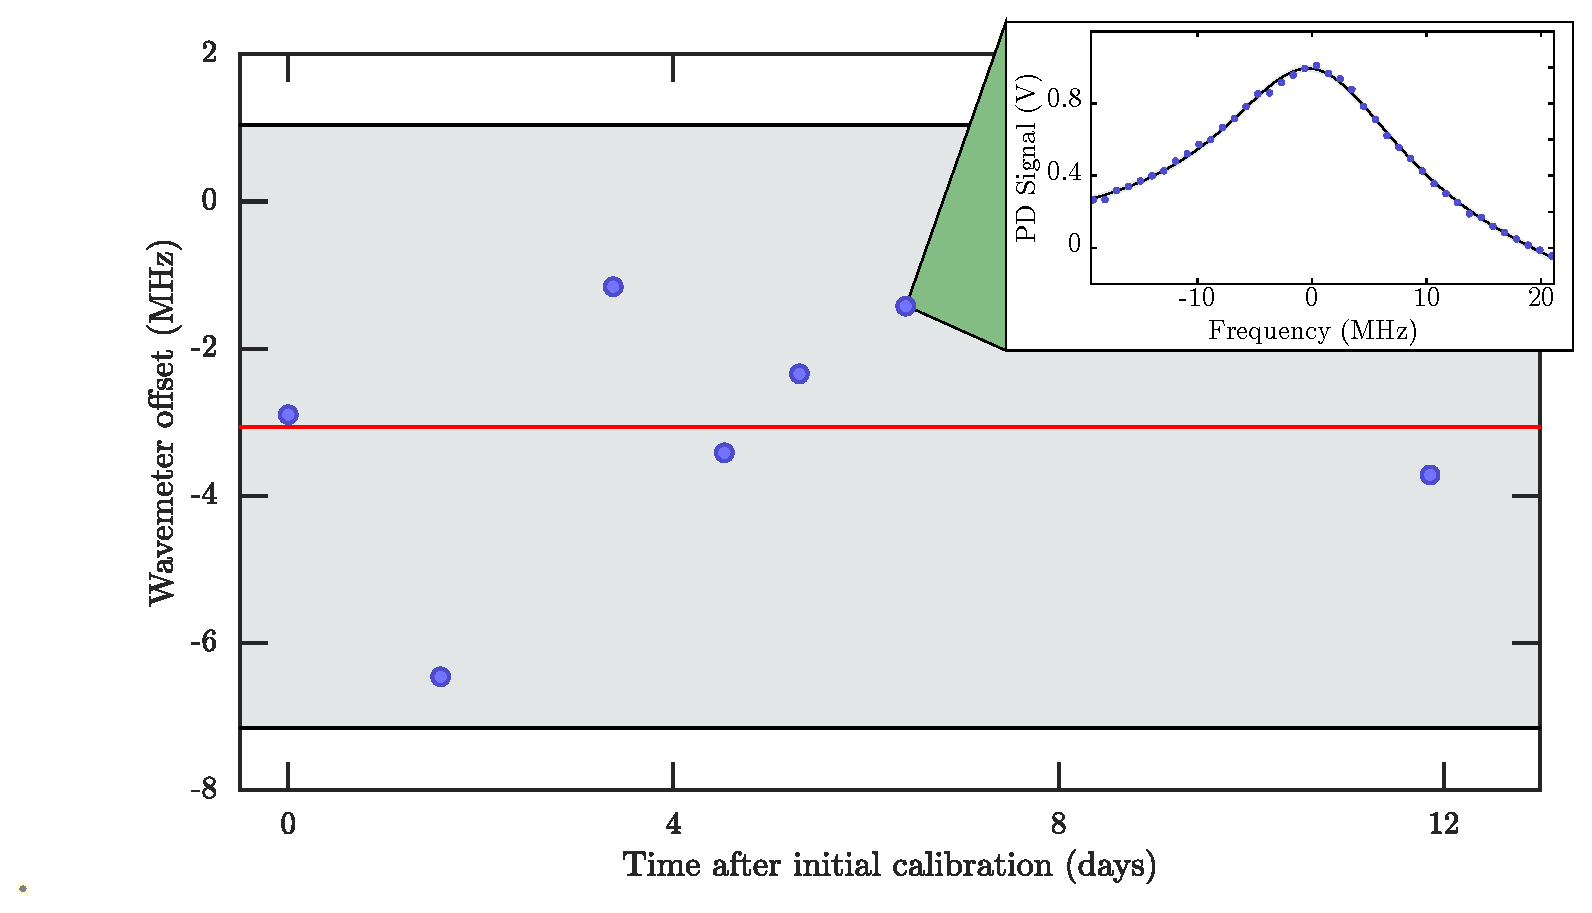
\includegraphics[width=0.7\textwidth]{SOMs/wm_err}
    \caption{Measured wavemeter offset versus time. Blue circles mark empirical data, with the red center line showing the mean of the data \(-3.01\)~MHz, and the black lines and shaded region indicating an uncertainty of \(4.1\)~MHz, which arises from the specified manufacture error and the distribution of the data. Standard deviation of the points is 1.7~MHz. Inset shows a single measurement using a fit of a Lorentzian with a second order polynomial background model to the cesium saturated absorption spectroscopy  of the \(6^2S_{\nicefrac{1}{2}}, F=4\) to the \(6^2P_{\nicefrac{3}{2}}, F=4\) and \(6^2P_{\nicefrac{3}{2}}, F=5\)  crossover line, with the measured frequency (from the wavemeter) offset by \(351,721,835.0\)~MHz, the measured frequency of Tanner and Wieman \cite{pmid9900545}.}
    \label{fig:wm_model}
\end{figure}
%{\color{red} (k adjust and clarify expand, maybe move plot to calibration section)}


\textbf{Probe Beam:} The probe beam consists of a Gaussian beam focused down, over a $\sim$700~mm distance, to a spot with a \(16\)~\(\mu\)m beam waist and Rayleigh range of \(91\)~\(\mu\)m, relative to the mean width of the atoms \(8\)~\(\mu\)m. See Fig.~\ref{fig:BEAM_WAIST} for beam profile along the axis of the probe beam, along with a fit to the spot size of the form \(w(z) = w_0 \sqrt{1+(z/z_R)^2}\) is shown in red, where \(w_0=16\)~\(\mu\)m is the beam waist, and \(z_R=91\)~\(\mu\)m is the Rayleigh range. The probe beam power averages \(31\)~mW with a standard deviation of \(4\)~mW, which gives an intensity at the focus of \(3.86 \times 10^7\)~W/m\(^2\). The atoms are exposed to the beam for a 20~\(s\) period.

\textbf{Apparatus:} The laser used was an M squared SolsTiS, a widely tuneable (700 to 1000 nm) Ti:Sapphire laser, with an M squared ECD-X doubling cavity (providing light in a 350 to 500 nm range). The laser was stabilised at a specific frequency via a proportional-integral-derivative (PID) feedback loop between a HighFinesse/\r{A}ngstrom WS8-2 wavemeter, measuring the laser's output, and the lab computer which controlled the scanning cavity within the SolsTiS. The power of the probe beam was measured just before the experimental chamber over time via the use of a photodiode, in order to calibrate the final signal with respect to incident power. 

%\subsection{Calibration of the Wavemeter}
% graph of wm drift and the interp model
% Wavemeter  uncertainty of 4.0 MHz

\textbf{Calibration of the Wavemeter:} The wavemeter was periodically calibrated by using saturated absorption spectroscopy in a cell with the non-doubled light (700 to 1000~nm) to perform  measurement of a known cesium crossover transition from \(6^2S_{\nicefrac{1}{2}}, F=4\) to between \(6^2P_{\nicefrac{3}{2}}, F=4\) and \(6^2P_{\nicefrac{3}{2}}, F=5\). This reference transition was constrained to be \(351,721,835.0(1)\)~MHz, equivalently \(852.3566870(3)\)~nm, by the measurement of Tanner and Wieman \cite{pmid9900545}. The reason this particular transition was chosen as a reference was that after applying the doubling cavity the light from this transition is \(\sim\)1.5~nm below the theoretically expected and experimentally measured wavelength of the transition of interest. From the manufacturer specifications we know that a calibration within \(2.0\)~nm gives the wavemeter an accuracy of \(2.0\)~MHz \cite{wstechnical}, however, as we are calibrating before the doubling cavity we must double this error to \(4.0\)~MHz.
The calibration shift in the wavemeter over time is shown in Fig.~\ref{fig:wm_model}. We correct for systematic wavemeter drift using the average of the calibrations, a shift of \(-3.01\)~MHz. The standard error in the distribution of the measurements was added to the fundamental wavemeter uncertainty to obtain a final uncertainty in this shift of \(4.1\)~MHz.  

\textbf{Detection:} The atoms are imaged in the far-field with full three dimensional resolution using an \(80\)~mm diameter micro-channel plate and delay line detector located \(\sim\)\(850\)~mm below trap centre, with a spatial resolution of \(\sim\)120~\(\mu m\) and temporal resolution of \(\sim\)3~\(\mu s\) \cite{Manning:10}.
 
 \textbf{Trap:} We use a magnetic bi-planar quadrupole Ioffe trap \cite{Dall2007}, which has trapping frequencies \(\omega_{(x,y,z)}/2\pi=\big(53.5(6),426.56(5),430.30(6)\big)\)~Hz. The trap frequencies of the magnetic trap were determined by inducing oscillations in the trap and then outcoupling portions of the atoms with RF pulses over time. From the measured 3D oscillations of the atoms we extract the trap frequencies.
 
 %The motion of the atoms represent an aliased trap frequency, which can be used to reconstruct the true trap frequency by varying the sampling trap frequency.
 
\textbf{Alignment of the Probe Beam:} We also use our trap frequency measurement technique as a tool to align the probe beam. We looked for a difference in the trap frequency between when the probe beam was and was not applied to the atoms. This frequency change is due to the dynamic polarizability the probe beam exerts on the atoms, adding an additional trapping potential that is approximately harmonic, which in turn purely depends upon the wavelength and the intensity of the light applied. Hence by keeping the wavelength fixed we were able to maximize the alignment on the atoms via maximizing the change in trap frequency.

\textbf{Fundamental light:} To ensure we are not observing a two photon process caused by the non-doubled fundamental light of the laser we use a range of measures: there is a filter which blocks wavelengths around the fundamental range just before the optic fiber that directs the light to the experimental chamber; the laser table and experimental chamber are completely isolated from each other; and we observe linear scaling of the signal amplitude with power in agreement with a single photon process.

\textbf{Radio Frequency Outcoupling:} The pulsed atom laser used to outcouple the atoms consists of a series of radio frequency  approximately 20~\(\mu\)s in length corresponding to a Fourier width of \(\sim 300\)~kHz \cite{Manning:10} which is much larger than the frequency width of the atomic distribution in the trap, which is given by the thermal energy distribution to be approximately \(10\)~kHz.

%We use a minimally-destructive spectrally broad RF pulse to remove \(\sim\)2\% of the atoms from the trap. The pulses are approximately 20~\(\mu\)s in length, and hence have a Fourier width of \(\sim 300\)~kHz \cite{Manning:10}, which ensures uniform outcoupling throughout the trap.

\section{Systematic Frequency Shifts}
\label{sec:freq_shifts}
\begin{figure}
    \centering
    \includegraphics[width=0.6\textwidth]{SOMs/ac_stark_shift_v3.png}
    \caption{Frequency center of the distribution relative to field free value \(f_r=700,939,271\)~MHz as a function of applied probe beam power. Note the reason the uncertainty of the data in this figure is less then implied by Fig.~\ref{fig:wm_model} is due to the shorter time scale these data points where taken over and that the systematic uncertainty in the wavemeter, which is the major source of uncertainty in Fig.~\ref{fig:wm_model}, does not effect the relative uncertainty of these points. See Sec.~\ref{sec:laser_linewidth} for more detail.}%, with error bars representing confidence interval in the fit
    \label{fig:ac_stark} %
\end{figure}
         \textbf{Zeeman shift:}
         The transition frequency is shifted by the Zeeman effect due to the energies of the initial and final states being shifted by different amounts due to external magnetic fields. The magnitude of the external field at the atoms is measured to be approximately 0.613(1)~G, by using a swept RF pulse to measure the Zeeman splitting between the \(\MetastableState, \,m_J=+1\) and \(m_J=0\) states. Note the magnitude of the magnetic field does not change between the direct detection and heating method. At field strengths of this size only the linear Zeeman effects will be relevant to our experimental precision. The frequency shift due to the linear Zeeman effect has the functional form 
         \begin{align}
             \Delta f &= \frac{\mu_B}{h} B (m_{J}^{e} g_{j}^{e} - m_{J}^{g} g_{j}^{g}),
         \end{align}
         where \(\mu_B\) is the Bohr magneton, \(h\) is the Planck constant, \(B\) is the magnetic field magnitude, \(g_{j}^{e}\) and \(g_{j}^{g}\) are the Land\'e \(g\)-factors of the excited and ground states respectively, and \(m_J^{e}\) and \(m_J^{g}\) are their respective magnetic quantum numbers. The atoms are initially in the \(\MetastableState, \, m_{J}^{g}=+1\) state with \(g_{j}^{g} = 2.0\) and are excited to the \(\UpperState, \, m_{J}^{e}=0\) state with \(g_{j}^{e} = 2.0\). Hence the Zeeman shift for our transition is \(\Delta f_{Zeeman} = - 1.715(3)\)~MHz.\\
         %The shift is really measured directly using RF tranistions from +1 to 0 states
         
         \textbf{AC Stark shift:}
         %Probe, RF knife
         For the tested experimental range the AC Stark shift is linearly proportional to the intensity of the probe beam at the atoms. Note we do not use any other light source in our trapping potential. As the focus of the probe beam is kept constant, the AC stark shift is linearly dependant on the total power in the beam. The power of the probe beam was measured using a calibrated photodiode. The frequency of the transitions was measured at a range of probe beam powers, as shown in Fig.~\ref{fig:ac_stark}. The data can then be used to linearly extrapolate to a field-free value of the frequency, with an uncertainty determined by the confidence interval of the fit. For the direct detection method we find a shift of \(\Delta f_{AC,Probe} = 8.6(1.5)\)~MHz and for the heating method \(\Delta f_{AC,Probe} = 5.9 (1.6)\)~MHz. The reason these values differ is the applied probe beam's focus size varied between the methods.
         % marked for removal
         %The radio frequency radiation present in the experimental chamber due to the RF knife will also cause an AC Stark shift. To determine the value of this shift we performed a scan with no RF knife applied and found the difference between the center of this scan and the predicted center from the linear extrapolation of the varying probe beam power, to isolate the RF AC stark shift from the probe beam stark shift. This difference then gives the shift due to the RF radiation as \(\Delta f_{AC,RF} = 0.94 (1.8)\)~MHz and as the RF field was kept constant for all other runs of the direct detection method this shift will be constant throughout. As no RF knife was present during the heating method this correction is not applied to its frequency value.\\
         
         \textbf{DC Stark shift:} For a multi-electron atom in either ground or low excited state in the presence of a weak static electric field its energy levels will be shifted as \(\Delta E = -\frac{1}{2} \alpha_s \mathbf{E}_{dc}^2\), where \(\alpha_s\) is the static polarisability of the atoms (in their current state) and \(\mathbf{E}_{dc}\) is the dc electric field of strength. As the electric field is kept constant the shift in frequency due to this effect is given by \(\Delta f_{DC} = -\frac{1}{2h} \Delta \alpha_s \mathbf{E}_{dc}^2\). For our case we can constrain from direct measurement that any static electric field in our experimental chamber has \(\mathbf{E}_{dc}<2\)~kV/m and \(\Delta \alpha < 6\times 10^{-50}\)~C\(^3\)m\(^3\)/J\(^2\) \cite{Kondratjev2010}, thus \(\Delta f_{DC}<10^{-10}\)~Hz. \\
         %\brycecom{feild is max 2kv/m, which is from 20eV over the 1cm sep between windows.}
         
         \textbf{Mean field shift:} The interactions between atoms in a BEC can also shift spectral lines, termed the mean field shift. For bosonic particles with sufficiently low temperatures such that only \(s\)-wave scattering will occur, which for the case of He\(^*\) corresponds to temperatures less than \(100\)~mK \cite{Julienne:89}, the density dependent mean field shift of the atomic energy level in a degenerate homogeneous system is given by \cite{PhysRevLett.81.3807}
         \begin{align}
             \Delta E = \frac{8 \pi \hbar^2 a n}{m},\label{eqn:mean_field_shift}
         \end{align}
         where \(a\) is the scattering length of the atoms in their current state, \(m\) is the mass of the atoms and \(n\) is the density of the atoms. Note that Eqn.~\ref{eqn:mean_field_shift} assumes only the elastic contribution to the collisional shift is relevant, which is valid for weak excitations \cite{PhysRevLett.81.3807}. The frequency shift induced in the spectroscopic transitions, neglecting inelastic processes, is hence
         \begin{align}
             \Delta f_{mf} = \frac{4 \hbar}{m} \left(n_f a_{f-f} + n_i a_{i-f} - n_f a_{i-f} - n_i a_{i-i}\right),
         \end{align} 
         where \(n_i\) and \(n_f\) are the density of the atoms in the initial and final states respectively and \(a_{i-i}\), \(a_{i-f}\) and \(a_{f-f}\) are the scattering lengths between the initial and initial, initial and final, and final and final states respectively. As the transition we are considering is extremely weak the density of the final state would be negligible, and thus \(\Delta f_{mf} \approx  \frac{4 \hbar n_i}{m} (a_{i-f} - a_{i-i})\). The scattering length of the \(\MetastableState-\MetastableState\) state collisions is of the order of \(10\)~nm \cite{PhysRevLett.96.023203,PhysRevLett.93.090409}, while the scattering length of the \(\MetastableState-\UpperState\) collisions can be calculated to be of order \(1\)~nm \cite{PhysRevA.48.546,PhysRevA.64.042710,TALU200183}. The average density of the atoms can be calculated from the atom number and the trap frequencies to be on the order of \(10^{19}\)~m\(^{-3}\). This gives us a mean field shift of the order \(\Delta f_{mf} \sim -10\)~kHz.\\
         
\begin{figure}[b]
    \centering
    \includegraphics[width=0.6\textwidth]{SOMs/cs_ac_stark_shift_v3.png}
    \caption{Measured center frequency of cesium calibration transition relative to the extrapolated theory free value \(f_r\) as a function of applied laser power. The dashed line represents linear best fit, with equation \(f_{rel} = -3.37\times 10^{-3} P\) where \(f_{rel}\) is the relative frequency in MHz and \(P\) is the applied power in \(\mu\)W. Note that like Fig.~\ref{fig:ac_stark} the uncertainty in these points are less than implied by Fig.~\ref{fig:wm_model} due to the different time scales they were taken over and as the systematic uncertainty does not affect the relative uncertainty of these points. See Sec.~\ref{sec:laser_linewidth} for more detail.}
    \label{fig:cs_stark_shift}
\end{figure}

         
         \textbf{Recoil shift:}
         Due to the conservation of momentum, when a photon is absorbed during an atomic transition the photon's momentum is imparted onto the atom. The momentum of the photon, and thus the change in momentum of the atom, is given by \(\Delta p = \frac{hf}{c}\), where \(f\) is the frequency of the absorbed photon and \(c\) is the speed of light. This increase in the kinetic energy of the atom must come from the photon, implying that there must be a shift in the energy of the photon in order to compensate for this imparted energy. The recoil shift of the photon's energy is \(\Delta E = \frac{1}{2m} \left( \frac{hf}{c} \right)^2\), where \(m\) is the atomic mass. The frequency of the transition was measured to be \(700,939,271(5)\)~MHz giving a recoil shift of \(0.273\)~MHz. As the relative uncertainty is on the order of parts per hundred-million the uncertainty within the recoil shift is well below \(1\)~kHz.\\
         
         
         \textbf{Cesium Cell offset:}  There are two main systematic shifts which occur in the cesium cell used to spectroscopically reference the wavemeter and laser: the AC Stark shift due to the probe laser and the vapour (or pressure) shift due to collisions within the cell. The AC Stark shift can be determined in the same manner as it was for the probe beam, by varying the power and measuring the change in the center frequency and then extrapolating to a theory free value, see Fig.~\ref{fig:cs_stark_shift}. The normal applied laser power is \(560\)~\(\mu\)W which gives an AC stark shift of \(\Delta f_{AC,Cs} = -1.9(4)\)~MHz. The pressure shift in the cell can be constrained using literature values, which state that the pressure shift is less than \(30\)~MHz/torr \cite{PhysRevA.80.062718,PhysRevA.82.042502}. The cell was at a temperature of \(84(1)\)~\(^\circ C\) which corresponds to a vapour pressure of \(2.00(2)\times 10^{-4}\)~torr \cite{1964JChEd..41R.590M}. Thus the vapour pressure shift in the cell is constrained to be \(\Delta f_{pressure} < 6 \times 10^{-3}\)~MHz.

\section{Polarisability effects on lineshape}
It can be see in Fig.~3 of the main text that the signal decays to a non-zero negative value, with a p-value of \(8.4 \times 10^{-7}\). This is most likely due to the repulsive dipole lensing caused by the probe laser, which leads to a slightly smaller proportion of atoms being detected.

We note that this may seem to imply that the dynamic polarisabilty (or ac-Stark shift) could effect the measured line shape. However, we believe this is not the case as the dynamic polarisability of the \(\MetastableState\) is approximately constant over the transition \cite{PhysRevA.88.052515,astapenko2013polarization,LeKien2013}, and hence so to is the approximate downward shift of the signal due to the dipole lensing. Furthermore the downward shift is small in comparison to the signal amplitude, the negative offset has a value of about \(2\%\) of the maximum signal. 

To see intuitively why the dynamic polarisability is approximately constant over the transitions linewidth consider that the dynamic polarisability of an atom \(\alpha(\omega)\), at a given frequency \(\omega\) and in a particular state, is give by the equation \cite{astapenko2013polarization,LeKien2013}
\begin{align}
    \alpha (\omega) &= \frac{e^2}{m_e} \sum_n \frac{f_n}{\omega_n^2-\omega^2- i \omega \delta_n}
\end{align}
where we are summing over all possible electronic transitions, \(e\) and \(m_e\) are the charge and mass of an electron, \(\delta_n\), \(f_n\) and \(\omega_n\) are the linewidth, oscillator strength, and center frequency of each transition. From this we can see that the main contributing factor to a particular transitions effect on the polarisability, aside from its detuning is its oscillator strength.

The oscillator strengths \(\MetastableState \rightarrow 3^{3\!}P\) and \(\MetastableState \rightarrow 2^{3\!}P\) are approximately \(12\) orders of mangitude greater than that of the \(\MetastableState \rightarrow \UpperState\) transition.  The \(\MetastableState \rightarrow 3^{3\!}P\) and \(\MetastableState \rightarrow 2^{3\!}P\) transitions are hence the dominant contributions to the polarisability over the frequencies considered, even though these transitions are far detuned, and the effect of the \(\MetastableState \rightarrow \UpperState\) transition is washed out due to it being highly forbidden.

The only other effect on the line shape due to the atomic polarisability is the Auter-Towns effect, which depends purely on the Rabi frequency \(\Omega\) \cite{PhysRevA.73.043416,CohenTannoudji1996}. The Rabi frequency is given by \(\Omega=\alpha E_{dc} \varepsilon_0\) \cite{PhysRevA.73.043416}, where \(\alpha\sim 2.45 \times 10^{-6}\)~Hz/(V/m)\(^2\) is the Stark polarisability, \(E_{dc}\) is the dc electric field amplitude (which can be constrained to be less than \(2\)~kV/m as described above), and \(\varepsilon_0\) is the ac electric field strength, which is \(\sim10^3\)~kV/m at the focus. We can hence constrain the Rabi frequency to be \(\Omega < 5\)~kHz, which is negligible compared to our linewidth, and hence we expect to see no Auter-Towns effect, which is what we observe.

\section{Details of Heating Method}

\begin{figure}[t]
    \centering
    \begin{subfigure}[t]{.5\textwidth}
        \centering
        \caption{}
        \includegraphics[width=1.15\textwidth]{SOMs/tof_heating_v2.png}
        \label{fig:tof}
    \end{subfigure}%
    ~ ~ ~ ~ ~ ~ ~
    \begin{subfigure}[t]{.5\textwidth}
        \centering
        \caption{}
        \includegraphics[width=0.9\textwidth]{SOMs/tof_pulse_v2.png}
        \label{fig:pulse}
    \end{subfigure}
    \caption{(a) Time of flight profile for the heating method consisting of 95 outcoupled atomic pulses. The outcoupled atoms arrive at the detector in pulses, signified by the peaked structure of the profile. Arrival time is measured from when the first outcoupling pulse is applied. (b) Zoom in of the first pulse, with the solid black line representing count rate over time and the dashed red line indicating a Gaussian fit. This particular fit has parameters \(t_0=1.756(1)\)~s, \(\sigma_t = 0.0051(1)\)~s (equivalent to \(T=1.21(2)\)~\(\mu\)K), and \(C_0 = 96(2)\)~kHz.}
\end{figure}

%The heating method uses a novel temperature method in order to calibrate the transition strength. 

Fig.~\ref{fig:tof} displays the number of counts detected versus time, with a broadened radio frequency pulse applied to the trapped atoms every \(240\)~ms corresponding to the peaks present in the profile. If we zoom in on a particular peak (Fig.~\ref{fig:pulse}) we can see it has a distinctive Gaussian profile. 
%e ballistic expansion of a cloud of trapped atoms falling under the influence of gravity. Using a simple coordinate transformation, we derive an analytical expression for the time-of-flight signal.
From Yavin \textit{et al.} \cite{Yavin2002} we know that the expected time of flight probability density profile for a ballistic expansion of particles from a point source is
\begin{align}
    n(t) &= A \pi v_0^2 \left( \frac{\frac{1}{2}gt^2 + d }{t^2}\right) \exp \left( - \frac{(\frac{1}{2}gt^2 - d )^2}{v_0^2 t^2}\right), \label{eqn:tof_den_int}
\end{align}
where \(d\) is the fall distance from the trap to the detector, \(A = (m /2 \pi k_B T)^{3/2}\), \(m\) is the mass of a particle, \(k_B\) is the Boltzmann constant, \(v_0 = \sqrt{2 k_B T/m}\) is the most probable velocity, and \(g=-9.81\)~m/s\(^2\) is the acceleration due to gravity.If the spread of the peak is small in time we can simplify Eqn.~\ref{eqn:tof_den} by approximating it as a Gaussian
\begin{align}
    n(t) &\approx A \pi v_0^2 \left( \frac{1}{2}g + \frac{ d }{t_f^2}\right) \exp \left( - \frac{(t - t_f )^2}{ 2 \left(\frac{2}{g} \sqrt{\frac{k_B T}{m}}\right)^2}\right) \label{eqn:tof_den},
\end{align}
where \(t_f = \sqrt{\frac{2 d}{g}}\) is the expected fall time for particles with zero velocity.
%This is because the probability density function for the velocities of particles following a Maxwell-Boltzmann distribution is given by
% \begin{align}
%     p(v) &= \left(\frac{m}{2\pi k_B T} \right)^{\nicefrac{1}{2}} e^{-\frac{mv^2}{2k_BT}} \label{eqn:max_boltz},
% \end{align}
%and ballistic kinematics relates the arrival time \(t\) to the particles vertical velocity \(v_z\) by the relation \(v_z(t) = d/t - \frac{1}{2} g t\), where \(d\) is the fall distance from the trap to the detector and \(g=-9.81\)~m/s\(^2\).
Thus we fit a Gaussian to the count rate distribution in time \(C(t)\) of the form,
\begin{align}
    C(t) &= C_0 e^{-\frac{(t-t_0)^2}{2\sigma_t^2}},
\end{align}
where \(C_0\) is the peak count rate, \(t_0\) is the center time of the distribution (the time of arrival for particles with zero initial vertical velocity), and \(\sigma_t\) is the standard deviation. From Eqn.~\ref{eqn:tof_den} we have \(\sigma_t = \frac{2}{g} \sqrt{\frac{k_B T}{m}}\).
%For small time perturbations about \(t_0\) we can expand the relation between the vertical velocity and arrival time to linear order, giving \(v_z(t) \approx -(t-t_0) g \). So the standard deviation in time \(\sigma_t\) is related to the standard deviation in velocity space \(\sigma_v\), as \(\sigma_v \approx - \sigma_t g\). 
Rearranging we obtain,
\begin{align}
    T &= \left( -g \sigma_t/2\right)^2 \times \frac{m_{He}}{k_B}
\end{align}

%Note that it can be seen in Fig.~\ref{fig:pulse} that there is a slight skew in the distribution towards the earlier times, or upwards velocities. This effect is most likely caused by a combination of atoms rescattering after leaving the BEC and possible mean field effects between atoms immediately after the RF pulse. 

From the fits of each pulse we extract the temperature versus time (see Fig.~\ref{fig:heating_fig}) and fit a line to this data, the gradient of which gives us the heating rate. The comparison of the heating rate with the probe applied to a reference then gives us a measure of the temperature increase purely due to photon absorption.

\begin{figure}
    \centering
    \includegraphics[width=0.6\textwidth]{SOMs/heating_fig_v3.png}
    \caption{Measured temperature versus arrival time for a particular run of the heating method with the probe beam applied (dashed green) and the probe beam blocked as a reference (solid blue). Each individual point on the plot corresponds to an individual pulse, see Fig.~\ref{fig:tof} and Fig.~\ref{fig:pulse}. }
    \label{fig:heating_fig}
\end{figure}

\section{Laser linewidth determination}
\label{sec:laser_linewidth}
To produce an independent estimation of the laser linewidth we employ spectroscopy of two cesium transitions. For determination of line-width up to $\sim$10~ks we use measurements of the two photon cesium $6^{2}S_{1/2} (F=4) \rightarrow 8^{2}S_{1/2} (F=4)$ transition at 364.5~THz (822.5~nm) which we detect using blue florescence in the cesium cell (the same as used in the wavemeter calibration as described in Sec.~\ref{sec:exp-details}) with a photonmultiplier tube (PMT) \cite{Fendel:07,Wu:13}. 

\begin{figure}
    \centering
    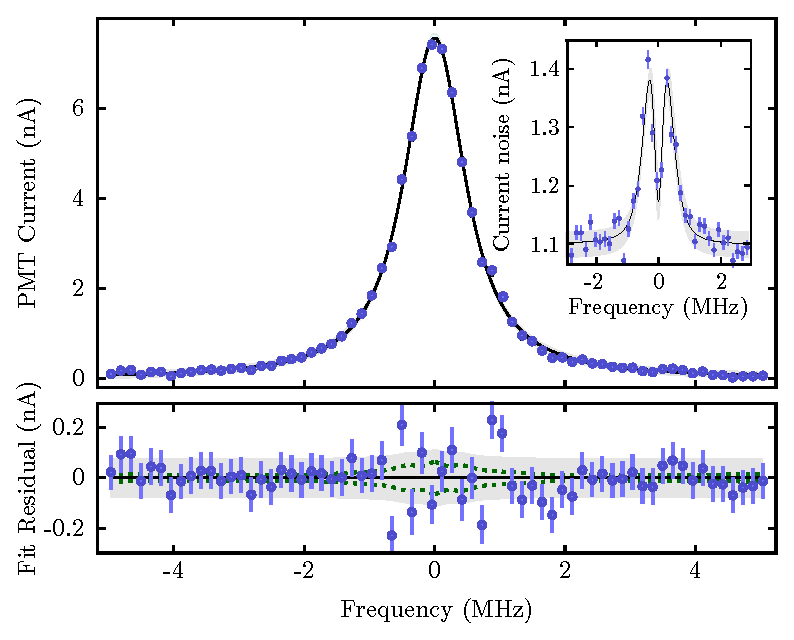
\includegraphics[width=0.6\textwidth]{SOMs/2p_scan_single}
    \caption{(Top) Example of a single scan across the two photon transition. Data points are marked in blue circles and Voigt fit is shown as the black line (error bars are smaller than maeker at this scale). Fit parameters are $\sigma=0.18(3)$~MHz $\gamma=0.49(3)$~MHz sentence (error is the standard deviation over many measurements). Inset shows fit to the PMT current noise with a given laser frequency noise component of \(0.075(1)\)~MHz. (Bottom) Residuals of the fit model, with shaded region shows one standard deviation of the observation error model and dashed lines are one standard deviation in the fit model. Current offset and fit frequency have been subtracted. Data shown here is acquired over \(75\)~s. }
    \label{fig:2p_scan_single}
\end{figure}

We acquire data by adjusting the set-point of our wavemeter feedback system and measuring the PMT current produced. We fit the observed transition with a Voigt profile, a convolution of a Gaussian with standard deviation \(\sigma\) and Lorentzian with  scale parameter \(\gamma\), as shown in Fig.~\ref{fig:2p_scan_single} with fit parameters $\sigma=0.18(3)$~MHz and $\gamma=0.49(3)$~MHz sentence (error is the standard deviation over many measurements). Note that the Lorentzian FWHM is within error of the predicted value of $\gamma=0.48$~MHz corresponding to the combined effect finite upper state lifetime ($\gamma=0.46$~MHz) and transit time broadening \cite{Fendel:07}. From this we can constrain the laser linewidth over timescales of the scans ($\sim$70~s) to be $\sigma\approx0.18(3)$~MHz and $\gamma<0.03$~MHz corresponding to the Gaussian and Lorentzian components of the un-doubled (red) probe laser system.
 % refit the measured PMT current vs set frequency, the Gaussian component  $\sigma=0.18(3)$~MHz and the Lorentzian is  $\gamma=0.49(3)$~MHz averaged across \(\sim\)10~h of scans. Note that the Lorentzian FWHM is within error of the predicted value of $\gamma=0.48$~MHz corresponding to the combined effect finite upper state lifetime ($\gamma=0.46$~MHz) and transit time broadening \cite{Fendel:07}. From this we can constrain the laser linewidth over timescales of the scans ($\sim$70~s) to be $\sigma\approx0.18(3)$~MHz  and $\gamma<0.03$~MHz corresponding to the Gaussian and Lorentzian components of the probe laser.
 
%  It is also possible to use the measured intensity noise along with a model to extract the laser frequency noise in the frequency range of \(2\)~Hz to \(3.5\)~kHz. The model combines a frequency noise term, a shot noise term, and a constant background noise. The frequency noise is multiplied by the magnitude of the frequency derivative of the Lorentzian component found from the average current fit. We found that the shot noise in the signal dominates over the negligible intensity noise in the laser. The average over the dataset is $0.07(1)$~MHz.
% \begin{align}
%     \sigma_{\mathrm{short}}^2=\left(\sigma_f \left| \frac{\partial L(\omega) }{\partial \omega} \right| \right)^2 + \left( \sigma_p \sqrt{V(\omega)}\right)^2+\sigma_b^2
% \end{align}
It is also possible to obtain an independent measurement of the laser frequency noise by using the noise in the PMT current as a function of the frequency. A strong component of this noise is from the transduction of laser frequency noise through the derivative of the line profile into the PMT current noise, which we define as the standard deviation of the measured PMT current. We use a model which combines this mechanism along with shot noise and background terms (in quadrature). The amplitude and center frequency used in these terms are fixed from the fit to the mean current. The result of one such fit is shown in the inset of Fig.~\ref{fig:2p_scan_single}. From this we get a laser frequency noise of $0.07(1)$~MHz between 2~Hz and 3.5~kHz. 

To find the contribution to the laser linewidth from drifts at timescales greater than the scan duration we introduce an estimator of the standard deviation \(\sigma^{2}(f(t),T,\tau)\) over integration duration $\tau$, which uses the center frequency \(\mu\) from the fits to multiple scans over about 10~h,
\begin{align}
    \sigma^{2}(f(t),T,\tau)&=\frac{1}{\tau}\int_{T}^{T+\tau}   (f(t)-\mu(f(t),T,\tau))^2 dt \\ 
    \mu(f(t),T,\tau)&=\frac{1}{\tau}\int_{T}^{T+\tau}  f(t) dt
\end{align}
% To get to longer timescales i use the center frequency from the fits to multiple scans over about 10~h.
% I then compute the standard deviation over varying size $\tau$ long chunks of the data. To see how the standard deviation in the laser frequency changes over time.

\begin{figure}
    \centering
    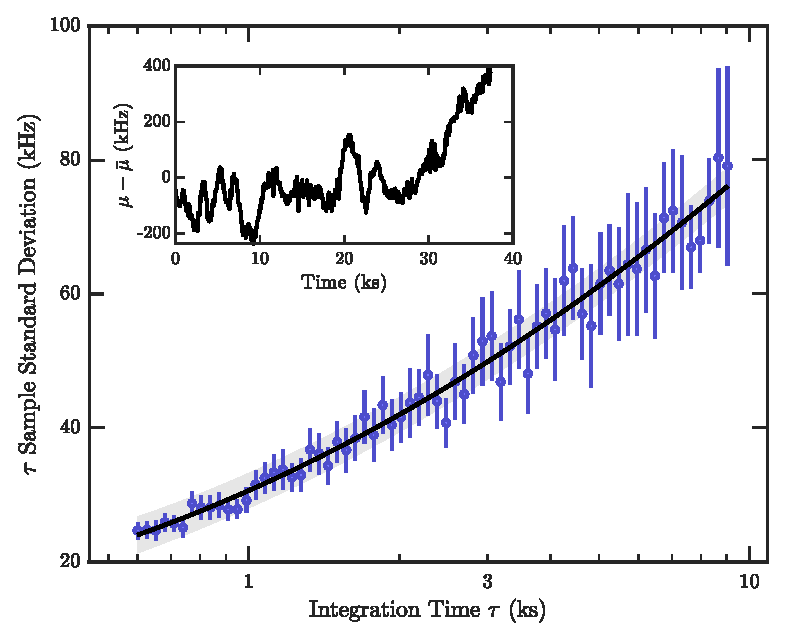
\includegraphics[width=0.6\textwidth]{SOMs/tau_sample_std_inset}
    \caption{Dependence of the standard deviation of the scan fit center frequency ($\mu$) with integration time $\tau$. Fit is a second order polynomial in log space $\sigma_f(\tau)=o+g\log_{10}{(t/1s)}+c\log_{10}{(t/1s)}^2$ with $o=66$~kHz, $g=-60(20) \mathrm{kHz}$, and $c=15(3) \mathrm{kHz}$. Inset shows the values of $\mu$ about the mean.}
    \label{fig:2p_tau_sd_dep}
\end{figure}

From Fig.~\ref{fig:2p_tau_sd_dep} we see a monotonic increase in the variation in the laser frequency. We cannot extrapolate from 10~h that these scans were taken over, to the 12 days that the main transition data was taken over. To this end we use two separate methods to estimate the effective laser linewidth at these time scales. 

In order to support the accuracy of this measurement we can use the cesium (SAS) calibration data as seen in Fig.~\ref{fig:wm_model}, and described in Sec.~\ref{sec:exp-details}. The standard deviation of this data is \(1.7(5)\)~MHz. To obtain the laser linewidth we combine in quadrature with the Gaussian component of the the short term laser linewidth \(0.36(6)\)~MHz (converted to the blue) giving \(1.7(5)\)~MHz, which is within error of the Voigt predicted Gaussian linewith for both sets of data. Here we have neglected the Lorentzian contribution which we have previously constrained to be $\gamma<0.06$~MHz.

For are main method we perform a Voigt fit directly to the data which gives a Guassian component of \(\sigma=1.9(4)\) for the direct detection method and \(\sigma=1.6(9)\) for the heating method.

% Now we can be confident of the laser linewidth integrated over the entire data acquisition.

%From Fig.~\ref{fig:2p_tau_sd_dep} we find that the predicted linewidth contribution at 16 days is $0.28(4)$~MHz (red). Combining this linewidth in quadrature with that measured in the Voigt fit gives the best estimate of the long term linewidth at \(0.33(7)\)~MHz on the non-doubled (red) side. Thus we find the effective laser linewidth on the measurement side to be \(0.66(14)\)~MHz.
% From this we see a monotonic increase in the variation in the laser frequency, unfortunately it is hard to extrapolate from 10h that these 2p scans were taken over to the 12 days that the forbidden transition data was taken over. To this end we use the cesium (SAS) calibration data that was taken during the forbidden data run.

% The standard deviation of this data is 1.7(5)~MHz (in the blue). To get the laser linewidth we combine in quadrature this with Gaussian component of the the short term laser line width 0.36(6)~MHz (converted to the blue) to get 1.7(5)~MHz. Now we can be confident of the laser line-width integrated over the entire data acquisition. Here i have neglected the Lorentzian contribution which we have previously constrained to be $\gamma<0.06$~MHz (converted to the blue).


\section{Theoretical Value of the excited state lifetime of the \(\UpperState\) state in helium}
The excited state lifetime is the average amount of time an atom will remain in a particular excited state before decaying to a lower energy state. The state lifetime \(\tau_u\) can be calculated for a given state \(u\) from the Einstein \(A\) coefficients of all transitions to lower lying states,
\begin{align}
    \tau_u &= \frac{1}{\sum_l A_{ul}},
\end{align}
where \(A_{ul}\) denotes the Einstein \(A\) coefficient for the transition between the upper \(u\) and the lower state \(l\). For the \(\UpperState\) state of helium the major contributions to the state lifetime are from the transitions to the \(\MidState\) states, which have respective Einstein \(A\) coefficients \(J=0\) \(A = 3.095(9)\times 10^{6}\)~\(\text{s}^{\text{-}1}\), \(J=1\) \(A = 9.28(3)\times 10^{6}\)~\(\text{s}^{\text{-}1}\), and \(J=2\) \(A = 1.55(5)\times 10^{7}\)~\(\text{s}^{\text{-}1}\) \cite{NISTASD}. Hence the theoretically expected state lifetime of the \(\UpperState\) state is \(\tau = 35.9(2)\)~ns.

\section{Experimental determination of Excited state lifetime}

The scattering probability distribution in frequency space of an individual transition has a fundamental limit of a Lorentzian distribution, whose linewidth, or more precisely full width half maximum (FWHM), \(\Gamma\) is related to the state lifetime of the excited state of the transition \(\tau\) by \(\tau = 1/(2\pi \Gamma)\). 

Due primarily to the finite laser linewidth, and Gaussian profile, of the probe laser the measured signal of the transition takes the form of a Voigt distribution. In order to extract the underlying Lorentzian profile of the transition we fit a Voigt profile to the measured data (see Fig.~\ref{fig:427nm_signal} and Fig.~\ref{fig:427nm_signal_heating} respectively in main text). We ensure that the Gaussian component of the Voigt profile is largely produced by the laser line profile as described in Sec.\ref{sec:laser_linewidth}. The Voigt profile hence directly gives the Lorentzian linewidth, which we find to be \(\Gamma_d = 3.2(10)\)~MHz for the direct detection method, and \(\Gamma_h=4(3)\)~MHz for the heating method, with the uncertainties given by the confidence interval of the respective fits. This gives us our value for the excited state (\(\UpperState\)) lifetime of \(\tau = 50(16)\)~ns for the direct detection method and \(\tau = 40(30)\)~ns for the heating method.

The other primary source of broadening is the mean field effect, however this is negligible compared to the laser linewidth. An approximate value for the mean field broadening can be obtained from the mean field shift calculated in Sec.~\ref{sec:freq_shifts}, hence for both methods we have \(\sigma_{mf} \sim 0.01\)~MHz, which converted to a FWHM is \(\Gamma_{mf} \sim 0.024\)~MHz, far below that of the laser linewidth.

%However, the experimentally measured values of the absorption linewidth, \(\Gamma_d = 5.74(28)\)~MHz and \(\Gamma_h=5(1)\)~MHz (see Fig.~\ref{fig:427nm_signal} and Fig.~\ref{fig:427nm_signal_heating} respectively in main text), is broadened by a number of factors; primarily our effective laser linewidth, and the mean field broadening, whose FWHM we denote \(\Gamma_{l}\), and \(\Gamma_{mf}\) respectively. 

%The effective laser line width was measured by taking the standard deviation of the calibration data, see Fig.\ref{fig:wm_model}, which can be converted to a FWHM assuming the distribution is Gaussian by multiplying by \(2\sqrt{2 \ln(2)}\) giving \(\Gamma_{l} = 1.9(7)\)~MHz, where the error is calculated from the standard error of the sample standard deviation of normally distributed data.
%The width of Doppler broadening can be calculated directly from the temperature of the BEC with \(\sigma_{th} = f_0\sqrt{\frac{k_B T}{mc^2}}\), where \(f_0\) is the frequency of the transition, \(k_B\) is the Boltzmann constant, \(T\) is the temperature, \(m\) is the mass of helium, and \(c\) is the speed of light. For the direct detection we have \(T\sim 100(50)\)~nK and hence \(\sigma_{th} = 0.03(15)\)~MHz and for the heating method we have \(T\sim 1000(100)\)~nK and hence \(\sigma_{th} = 0.042(5)\)~MHz.


%The broadening effects have Gaussian distributions, and hence when they convolve with our signal which has a Lorentzian distribution they form a Voigt distribution. Note that we fit a Lorentzian to our data rather than a Voigt function for technical ease, due to the broadening effects being small in comparison to the width of the signal, and hence the Lorentzian fit gives a reasonably accurate measure of the FWHM of the true Voigt distribution. The FWHM of a Voigt distribution is given approximately by \(\Gamma_V\approx 0.5346\Gamma_L+\sqrt{0.2166\Gamma_L^2+\Gamma_G^2}\) \cite{Olivero1977} where \(\Gamma_L\) and \(\Gamma_G\) are the FWHM's of the Lorentzian and Gaussian distributions being convolved. For the direct detection method we have \(\Gamma_V=5.74(28)\)~MHz and as the mean field contribution is negligible compare to the laser linewidth the broadening sources can be considered one Gaussian with FWHM \(\Gamma_G=1.9(7)\)~MHz. Inverting this relationship we obtain the FWHM of the true distribution \(\Gamma_L=5.0^{+0.6}_{-1.0}\)~MHz, which gives us our excited state lifetime of \(\tau = 33(6)\)~ns for the direct detection method. Following the same method for the heating method, with values \(\Gamma_V=5(1)\)~MHz and \(\Gamma_G= 1.9(7)\)~MHz, we obtain \(\Gamma_L=4.2^{+1.5}_{-2.0}\)~MHz and hence \(\tau = 40(20)\)~ns.

%, where we use the relation \(\Gamma_G=2\sqrt{2\log(2)} \sqrt{\sigma_{l}^2+\sigma_{th}^2}\) for two convolved Gaussians

%After accounting for this [\TODO{put this calc in appendix}] we get a a fundamental absorption line width of \(??\), corresponding to a state lifetime of \(??\)~ns[\TODO{calculate this value}], which is in ... [\TODO{comment on relation to theory value}]. The lifetime is also likely be shortened by in trap collisions. The collision rate within a BEC is well approximated by \(\gamma_c = n \bar{v} \sigma\), where \(n\) is the average density, \(\bar{v}=4\sqrt{k_B T}/\sqrt{\pi m}\) is the average collision velocity and \(\sigma\) is the collision cross-section \cite{dalibard1999collisional}. The transition rate will increase by the rate of collision per particle. For our experiment we have \(\gamma_c/N \sim 0.1\)~Hz which hence has a negligible effect on the state lifetime. 
 
 %absorption linewidth of \(\Gamma_\nu = 5.74(28)\)~MHz, to be \(1/(2\pi\Gamma_\nu) = 27.7()\)~ns. 
 
\section{Experimental determination of Einstein \(A\) coefficient}

%Run through the derivation of osc strength from heating/ direct detect

%To obtain an expression for the Einstein \(A\) coefficient that can be calculated from empirical data we start from a fundamental expression, Eqn.~\ref{eqn:A_main}, and convert it into an expression relating the amount of energy removed from the beam, which is directly related to the number of scattered photons, to the Einstein \(A\) coefficient. 

In this section we present a derivation of an expression for the Einstein \(A\) coefficient that is entirely dependant on empirical data and known quantities, starting from a fundamental expression, Eqn.~\ref{eqn:A_main}. First consider light with frequency \(f\) and intensity distribution \(I_{f}(x,y,z)\) propagating along the \(x\)-axis through some absorbent medium. The change in intensity at a particular point \(\delta I_{f} (x,y,z)\) over a small distance \(\delta x\) is given by the expression \cite{Huber1986}
\begin{align}
    - \delta I_{f} (x,y,z) &= k(f,x,y,z) I_{f} (x,y,z) \delta x \label{eqn:A_main},
\end{align}
where \(k(f,x,y,z)\) is the frequency and density dependant absorption coefficient. Let the total power in the light field at point \(x\) be \(P_{f}(x)\) and \(I_{f} (x,y,z) = P_{f}(x) \phi_I(x,y,z)\), where \(\phi_I(x,y,z)\) is a function that gives the distribution of the power over a given plane and has unit normalisation. We can hence integrate Eqn.~\ref{eqn:A_main} over the \(y\)-\(z\) plane, the plane perpendicular to the direction of light propagation, and obtain the change in power \(\delta P_f(x)\) over an infinitesimal distance \(\delta x\) is
\begin{align}
    - \delta P_{f}(x) &= P_{f}(x) \delta x \int \int  dy dz  \, k(f,x,y,z) \phi_I(x,y,z)\\
    \therefore - \frac{\delta P_{f}(x)}{P_{f}(x)} &= \delta x \int \int  dy dz \, k(f,x,y,z) \phi_I(x,y,z). \label{eqn:temp_1}
\end{align}
Both sides of Eqn.~\ref{eqn:temp_1} can be integrated to obtain,
\begin{align}
    - \int \frac{d P_{f}(x)}{P_{f}(x)} &= \int \int \int dx  dy dz \, k(f,x,y,z) \phi_I(x,y,z)\\
    -\log\left( \frac{P_{f}^+}{P_{f}^-} \right) &= \iiint_{all\, space} \, k(f,x,y,z) \phi_I(x,y,z) \label{eqn:temp_2},
\end{align}
where \(P_{f}^-\) is the power in the light field before moving through the medium, in a theoretical sense the power at \(x=-\infty\), and \(P_{f}^+\) is the power in the light field after the medium, \textit{i.e.} the power at \(x=+\infty\). Next we note that the integral of the absorption coefficient over the line shape of a transition is related to the Einstein \(A\) coefficient as follows \cite{Huber1986}:
\begin{align}
    \int_{line} k(f,x,y,z) df &= \frac{c^2}{8 \pi f_0^2} A_{ul} \, n(x,y,z),
\end{align}
where \(f_0\) is the center frequency of the transition, \(A_{ul}\) is the Einstein \(A\) coefficient for the transition between the states \(u\) and \(l\), and \(n(x,y,z)\) is the atomic density distribution at the point \((x,y,z)\). Therefore Eqn.~\ref{eqn:temp_2} can be written as
\begin{align}
   -\int df \log\left( \frac{P_{f}^+}{P_{f}^-} \right) &= \iiint_{all\, space} \, \frac{c^2}{8 \pi f_0^2} A_{ul} \, n(x,y,z) \, \phi_I(x,y,z) \label{eqn:temp_3},
\end{align}
where we have assumed the intensity distribution is frequency independent. To simplify Eqn.~\ref{eqn:temp_3} further, we assume that the power removed from the beam is small and so we can Taylor expand \(-\log\left( \frac{P_{f}^+}{P_{f}^-} \right)\) about \(1\) as \(-\log\left( \frac{P_{f}^+}{P_{f}^-} \right) \approx \frac{P_{f}^--P_{f}^+}{P_{f}^-}\). The difference between the initial and final powers is equal to the rate of photons scattered by the atoms multiplied by the energy of the photon, \(P_{f}^--P_{f}^+= h f \frac{dN_{scatter}}{dt}\). The number of scattered photons can be calculated from the frequency dependant heating rate due to the probe beam \(\frac{dT}{dt}(f)\), the heat capacity of the atoms, which for a thermal gas in a constant harmonic trap is \(C_b = 3 N k_B\) \cite{doi:10.1119/1.3417868}, and the average energy added to the gas by each photon \(E_p\), from the relation \(\frac{dN_{scatter}}{dt} = \frac{dT}{dt}(f) \frac{C_b}{E_p}\). We can simplify even further by utilising the relation \(n(x,y,z) = N \phi_N(x,y,z)\), where \(N\) is the total atom number and \(\phi_N(x,y,z)\) gives the atomic density distribution with unit normalisation. Combining we see Eqn.~\ref{eqn:temp_3} becomes,
\begin{align}
    \int df \frac{hf}{P_{f}^-} \frac{dT}{dt}(f) \frac{C_b}{E_p} &= \frac{c^2}{8 \pi f_0^2} A_{ul} \iiint_{all\, space} \,  \, \phi_N(x,y,z) \, \phi_I(x,y,z) \\
    \therefore A_{ul} &= \frac{24 \pi f_0^2 h k_B}{c^2 E_p} \frac{ \int df f \left(P_{f}^-\right)^{-1} \frac{dT}{dt}(f)}{\iiint_{all\, space} \,  \, \phi_N(x,y,z) \, \phi_I(x,y,z)}. \label{eqn:A_final}
\end{align}
The parameters in Eqn.~\ref{eqn:A_final} are all experimentally measured or determined as follows: \(f\) is measured by the HighFinness wavemeter, \(P_{f}^-\) is measured by a calibrated photodiode, \(\frac{dT}{dt}\) is extracted from the data as described in the heating method section, \(\phi_I(x,y,z)\) is measured via a camera, \(\phi_N(x,y,z)\) can be determined by the trapping frequency and temperature \cite{doi:10.1119/1.3417868}, \(E_p\) is the energy transferred to the cloud on average by the recoil momentum of the photons, and the remaining parameters are all known constants.

The energy transferred to the cloud from photon recoils can be estimated by \(E_p = \eta \frac{1}{2m} \left(\frac{h}{c}\right)^2(f_0^2 + f_1^2 + f_2^2)\), where \(\frac{1}{2m} \left(\frac{h f}{c}\right)^2\) is the energy of a single photon recoil for a given photon of frequency \(f\), \(f_0\), \(f_1\), and \(f_2\) are the frequencies for the the \(\MetastableState \rightarrow \UpperState\), \(\UpperState \rightarrow \MidState\), and \(\MidState \rightarrow \MetastableState\) transitions respectively, and \(\eta\) is the probability that an excited photon transfers its recoil energy to the cloud. Note that we can make the approximation that all excitations have the same photon recoil as the linewidth of the transition is negligible compared to its center frequency. To see that the average energy transferred to the atom from the three transitions is the sum of their respective photon recoils consider the momentum distribution after absorption and the two emissions, see Fig.~\ref{fig:k_dist}, the average momentum is hence given by the surface integral
%The reason for the factor of \(2\)in \(E_p\) is the extra photon recoils the atom receives from the photon emission due to the \(\UpperState \rightarrow \MidState\) and \(\MidState \rightarrow \MetastableState\) transitions.
\begin{align*}
    \avg{k^2} &= \frac{1}{4\pi k_1^2 \times 4\pi k_2^2}\int^{2\pi}_0 d \theta_1 \int^{\pi}_0 d \phi_1 \int^{2\pi}_0 d \theta_2 \int^{\pi}_0 d \phi_2 \, [\left(k_0 + k_1 \sin(\theta_1)\cos(\phi_1) + k_2 \sin(\theta_2)\cos(\phi_2)\right)^2+...\\
     &\, \, \, \, \, \, \, \, \left(k_1 \sin(\theta_1)\sin(\phi_1) + k_2 \sin(\theta_2)\sin(\phi_2)\right)^2+\left(k_1\cos(\phi_1) + k_2 \cos(\phi_2)\right)^2]k_1^2 \sin(\phi_1) k_2^2 \sin(\phi_2)\\
    &= k_0^2 + k_1^2 + k_2^2
\end{align*}
where \(k_i = 2\pi f_i/c\), is the wavenumbers for the respective transition. 

To calculate \(\eta\) we assume that all atoms which decay to a trapped state, \(24.07\%\) of excited atoms, thermalise with the cloud, and those that decay to an untrapped state have an additional probability of colliding with another atom in the BEC or cloud as the excited atom leaves. To determine this additional probability we perform a Monte Carlo simulation of an atom leaving the cloud. The procedure for this simulation is as follows, we randomly sample from the momentum distribution of the cloud, given by the trapping parameters and temperature, and from the momentum distribution produced by the three photon recoils due to the absorption from \(\MetastableState\) to the \(\UpperState\) excited state and then the decays to the \(\MidState\) and then \(\MetastableState\) states, see Fig.~\ref{fig:k_dist}. These momenta are then added together and the atoms initial position is also sampled from the distribution given by the temperature and trapping parameters. The atom is then propagated ballisticly under gravity. We then simulate the probability of the atoms colliding with another atom at a specific point using the atomic density distribution and the scattering cross section \(\sigma = 4 \pi a^2\) where \(a\) is the \(s\)-wave scattering length of the \(\MetastableState\) state. We then repeat this process many times to find the average probability of a collision, and hence thermalisation, with the cloud, which we denote \(\eta_c\). The total probability is hence \(\eta = 24.07\% + \eta_c\).

\begin{figure}
    \centering
    \includegraphics{SOMs/k_dist_v5.png}
    \caption{Cross section of the momentum distribution (in wavenumber space) of an atom after it has under gone the \(\MetastableState \rightarrow \UpperState\) (\(k_0\)), \(\UpperState \rightarrow \MidState\) (\(k_1\)), and \(\MidState \rightarrow \MetastableState\) (\(k_2\)) transitions. Note that three arrows show are meant to be representative of a particular possible outcome, and the circles are crosssection representations of spheres.}
    \label{fig:k_dist}
\end{figure}

\textbf{Error propagation for the Einstein \(A\) coefficient:} 
Eqn.~\ref{eqn:A_final} can be simplified as \(A=\frac{C I_1}{E_p I_2}\), with \(C=\frac{24 \pi f_0^2 h k_B}{c^2}\), \(E_p\) as defined above, \(I_1 = \int df f \left(P_{f}^-\right)^{-1} \frac{dT}{dt}(f)\) and \(I_2 = \iiint_{all\, space} \,  \, \phi_N(x,y,z) \, \phi_I(x,y,z)\).
Using regular propagation of uncertainty we find the uncertainty in \(A\), which we denote \(\delta A\), to be
\begin{align}
    \delta A &= A \sqrt{\left(\frac{\delta C}{C}\right)^2 + \left(\frac{\delta I_1}{I_1}\right)^2 + \left(\frac{\delta E_p}{E_p}\right)^2 + \left(\frac{\delta I_2}{I_2}\right)^2 }
\end{align}
Since the error in \(C\) is negligible we have \(\delta C =0\). We can propagate the error in \(I_1\) and \(I_2\) using bootstrapping techniques. The error in \(E_p\) is dominated by uncertainty in the Monte Carlo simulation, which can be estimated through the standard deviation of the output. With the above the error in \(A\) can hence be calculated.


%hyper-fine states
\section{Clebsch-Gordan coefficients}
The Clebsch-Gordan coefficients represent the angular momentum coupling between different atomic states. For our work they are relevant because the modulus squared of the  Clebsch-Gordan coefficient between two particular magnetic substates is equal to the relative intensity, or probability, of that transition in comparison to all other transitions between the two respective manifolds \cite{Krainov2019}. The relative transition strengths, normalised to the weakest allowed transition, between the \(^{3\!}S_1\) and \(^{3\!}P_{0,1,2}\) manifolds are given in Tab.~\ref{tab:clebsch_gordan} \cite{metcalf1999laser}. Given that the excited particle is initially in the \(\UpperState, \, m_J=0\) state and the transitions from this state are dominated by decays to the \(\MidState\) states, and then from those states the transitions are dominantly towards the \(\MetastableState\) state, we can calculate the probability of an atom decaying to each magnetic sub state from Tab.~\ref{tab:clebsch_gordan}. The initial relative transition probabilities from the \(\UpperState, \, m_J=0\) state are given by the second row of Tab.~\ref{tab:clebsch_gordan}, and the exact fraction can be obtained by normalising the row by its sum \(18\). The transitions from the \(\MidState\) magnetic sub states to the \(\MetastableState, \, m_J=(+1,0,-1)\) sub states are given by the column of each relevant state (specifically all states except \(2^{3\!}P_{2}, \, m_J=\pm2\) as \(m_J\) can at most change by one), and again the fractions can be obtained by normalising each column by its total \(6\). From this we obtain the fraction of atoms that decay down each of the possible paths, and after summing the fractions which lead to each final state we obtain the total fraction that end up in each \(\MetastableState, \, m_J=(+1,0,-1)\) state as \(\left(\frac{26}{108},\frac{56}{108},\frac{26}{108}\right)\) or as approximate percentages \(\left(24\%,52\%,24\%\right)\).
%\renewcommand\arraystretch{1.3}
\begin{table}[]
    \centering
    \begin{tabular}{@{\extracolsep{\fill}}>{\centering}p{0.06\textwidth} |
    @{\extracolsep{\fill}}>{\centering}p{0.06\textwidth} |
    @{\extracolsep{\fill}}>{\centering}p{0.07\textwidth} |
    @{\extracolsep{\fill}}>{\centering}p{0.07\textwidth}
    @{\extracolsep{\fill}}>{\centering}p{0.07\textwidth}
    @{\extracolsep{\fill}}>{\centering}p{0.07\textwidth}|
    @{\extracolsep{\fill}}>{\centering}p{0.07\textwidth}
    @{\extracolsep{\fill}}>{\centering}p{0.07\textwidth}
    @{\extracolsep{\fill}}>{\centering}p{0.07\textwidth}
    @{\extracolsep{\fill}}>{\centering}p{0.07\textwidth}
    @{\extracolsep{\fill}}>{\centering\arraybackslash}p{0.07\textwidth}}
    \toprule
    \toprule
         \(^{3\!}S_1\) &\multicolumn{10}{c}{\(^{3\!}P_J\)}  \\
         \hline
         \(m_J\)& J & \multicolumn{1}{c|}{\!0} & \multicolumn{3}{c|}{\!\(1\)} & \multicolumn{5}{c}{\!2} \\
         & \(m_J\)&0&\(+1\)&0&\(-1\)&\(+2\)&\(+1\)&\(0\)&\(-1\)&\(-2\)\\
         \hline
         \(+1\)& &\(2\)&\(3\)&\(3\)&\(-\)&\(6\)&\(3\)&\(1\)&\(-\)&\(-\) \\
         \(0\)& &\(2\)&\(3\)&\(0\)&\(3\)&\(-\)&\(3\)&\(4\)&\(3\)&\(-\) \\
         \(-1\)& &\(2\)&\(-\)&\(3\)&\(3\)&\(-\)&\(-\)&\(1\)&\(3\)&\(6\)\\
    \bottomrule
    \bottomrule
    \end{tabular}
    \caption{Transition strengths in the D-line of He* obtained from the mod square of the  Clebsch-Gordan coefficient and normalised to the weakest allowed transition \cite{metcalf1999laser}. To obtain fractional transition rates divide the values in the relevant row or column by its respective total (\(18\) for rows and \(6\) for columns).}
    \label{tab:clebsch_gordan}
\end{table}

\section{RF Knife}

For the direction detection method a constant radio frequency field was applied to the atoms during the detection phase. The reason for this was to attempt to increase the detection efficiency of atoms which absorb a photon by both outcoupling some portion of atoms which decay back to the trapped \(\MetastableState,\, m_J=+1\) state, and lensing these atoms so that a higher proportion would land on the detector.

Consider that the two subsequent photon decays produce a momentum distribution which is a filled shell with a center translated by an outer radius equal to a 427~nm photon recoil. As the maximum magnetic field experienced by an atom oscillating in the magnetic trap is proportional to its maximum kinetic energy, by applying RF radiation tuned to the \(\MetastableState, m_J=1 \rightarrow 0\) transition for a given magnetic field strength we can selectively outcouple atoms with maximum kinetic energy above a threshold. Furthermore, as the trap does work on an atom the momentum space distribution of these outcoupled atoms is reduced in size, hence improving collection efficiency. Thus while only $\sim$24\% of atoms decay to the \(\MetastableState,\, m_J=+1\) state via this process they could theoretically significantly increase the total signal amplitude. The interplay between these two effects produce an optimum collection efficiency that depends on the particular momentum distribution and detector geometry.

It was found experimentally, however, that there was no statistically significant increase in the signal amplitude between the RF field applied and not applied. The exact reasons for this are unknown but we conjecture that the atoms scattering as they leave the trap and the RF not saturating the transition are the most likely contributing factors.

% \section{Sensitivity Metric}
% The measured number of background/dark counts for our detector system is \(130/s\). This allows our method to be extremely sensitive as we only need to detect 260 atoms\(/s\) to achieve a signal to noise ratio greater than \(2:1\).

% background for direct is largely dark counts
% background for heating largely background heating, from in trap effects

% We can calculate a sensitivity metric for this method, which indicates the weakest transitions, \textit{i.e.} smallest Einstein \(A\), this technique can detected for a given power, atom number, and interrogation time

% The sensitivity metric which we quote is defined as the transitions with the smallest Einstein \(A\), \(A_{min}\), that the given technique can detect for a given power, atom number and interrogation time. In order to understand how this is calculated consider a technique which is used to measure a transition with Einstein \(A\) Coefficient \(A_0\). If the technique produces a peak signal-to-noise ratio \(\sigma_{max}\) after interrogating \(N\) atoms for a total time \(t\) with power \(P\), from Poissionian statistics we can see that the signal-to-noise ratio should scale approximately as \(\sigma(N,t,P) \approx \frac{\sigma_{max}}{\sqrt{N t P}}\). Next we make the assumption that in order to detect a transition we require a signal to noise ratio of \(\sim 2:1\). Hence if our signal scales linearly with \(A_0\) we have
% \begin{align}
%     A_{min} (N,t,P) &= \frac{2A_0}{\sigma(N,t,P)}.
% \end{align}
% For the direct detection method we have \(\sigma_{max} = 25.96\) for \(N=1.7\times 10^6\) atoms, \(t=25\times215\)~s (as we interrogate for \(25\)~s for each of the total of \(215\) measurement shots), and \(P=26\)~mW. Thus \(A_{min}= 5\times10^{\text{-}10}\)~\(\text{s}^{\text{-}1}\) and \(A_{min} (N,t,P) = 8.3\times10^{\text{-}6}\)~\(\text{s}^{\text{-}1}\sqrt{\text{atom J}}\). 
% For the heating method \(\sigma_{max} = 7.83\) for \(N=1\times 10^7\) atoms, \(t=25\times188\)~s, and \(P=17.8\)~mW, thus \(A_{min} (N,t,P) = 5.2\times10^{\text{-}5}\)~\(\text{s}^{\text{-}1}\sqrt{\text{atom J}}\) and \(A_{min}= 1.79\times10^{\text{-}9}\)~\(\text{s}^{\text{-}1}\).

% For reference we find the weakest transitions the heating method could ideally detect, based upon the statistical uncertainty in the data and for our experimental conditions, to be \(A_{min} \sim 1.8\times10^{\text{-}9}\)~\(\text{s}^{\text{-}1}\) \cite{SOMs}. The absolute value of this fundamental limiting sensitivity is far below that of other techniques, which historically have had similar relative uncertainties of \(25\%\) to \(50\%\) but absolute uncertainties of \(\sim10^{3}\)~\(\text{s}^{\text{-}1}\) \cite{Whaling85,Pickering11}. 

\section{Sensitivity Metric}

We can define a metric in order to quantify the sensitivity of our measurement techniques in terms of minimum detectable Einstein A values. Our method is expected to have a signal to noise ratio (SNR) which is given by Poissionian statistics as,
\begin{equation}
    \mathrm{SNR}= \frac{A \sqrt{N t P \eta }}{S}  ,
\end{equation}
where $A$ is the Einstein \(A\) Coefficient, $N$ is the atom number, $\eta$ is the detector QE, $t$ is the integration time, $P$ is the beam power. The sensitivity $S$ is defined as the transition with the smallest Einstein \(A\) Coefficient ( \(A_{min}\)) that can be detected per square root of the previous signal scaling paramters
For the direct detection method we have \(\mathrm{SNR} = 26\) (for a single dataset ), \(N=1.7\times 10^6\) atoms, \(t=25\times215\)~s (as we interrogate for \(25\)~s for each of the total of \(215\) measurement shots), \(P=26\)~mW, and $\eta=0.09$. 
Thus we find the specific sensitivity to be \(S\approx 1\times10^{-6}\)~\(\text{s}^{-1} \sqrt{s\cdot W}\) and the minimum detectable value ($\mathrm{SNR}=1$) for our experiment at \(A_{\mathrm{min}}^{\mathrm{direct}} \approx 7 \times10^{-11}\)~\(\text{s}^{\text{-}1}\) (\(1/A \approx 470\)~years)  for a combined day of interrogation. 
% time specific sensitivity 2e-8 s^-1 \sqrt{s}
The heating method is less sensitive with \(\mathrm{SNR} = 8\),  \(N=1\times 10^7\) atoms, \(t=25\times188\)~s, and
\(P=17.8\)~mW, giving \(S\approx 8\times10^{-6}\)~\(\text{s}^{\text{-}1} \sqrt{s\cdot W}\). The corresponding minimum detectable value ($\mathrm{SNR}=1$) for this method is \(A_{\mathrm{min}}^{\mathrm{heat}} \approx 2 \times10^{-10}\)~\(\text{s}^{\text{-}1}\) (\(1/A \approx 160\)~years) for a combined day of interrogation. 
Both methods are currently limited by technical effects, the direct detection by the by the dark count rate of the detector system \(\sim130/s\) and the heating rate by the background heating rate of trapped atoms. These current limits could be improved on by using MCPs with lower radioisotope levels for lower background count rate and using a weaker trap where the heating rate is lower. 


%\begin{table}[t]
    %\centering
    %\begin{tabular}{|l|r|}
    %\hline
        %Type & Value (kHz) \\
        %\hline
        %Statistical & 80\\
        %Wavemeter uncertainty & 4000\\
        %All the shifts & ??\\
        %\hline
        %Total (in quadrature) &\\
        %\hline
    %\end{tabular}
    %\caption{Error budget of frequency \com{may make more sense to merge into other table, keep in~MHz}}
    %\label{tab:error_budget}
%\end{table}
% \1 Shifts of frequency
% \2 DC stark
% \(DC_{shift}=-1/2(\alpha^{3,0}_S-\alpha^{2,0}_S)F^2\) \cite{Delone_1999}
% \2 AC stark
% for energy dif=\(-1/4\)diff in dynamic polarizability \(F^2\) [\TODO{1083 and the probe beam}]



%\subsection*{Moved from main text}

 
 
 %Around 75.93\% will end up in an untrapped state (primarily \(\MetastableState m_J=0,-1\) though a very small proportion some will also end up in the \(2^1S_0\) and \(1^1S_0\) true ground state). These atoms thus leave the trap immediately and fall under the influence of gravity, and may scatter again while leaving the BEC with probability of xx \% [\TODO{monte carlo}]. After falling 120~\(\mu\)m approximately xx \% [\TODO{calc}] land on the detector according to our Monte Carlo simulation [\TODO{do it}].
 
% The remaining atoms (24.07\%) will return to the trapped \(\MetastableState, m_J=+1\) state. These atoms momenta will now lie upon a convolution of the two spheres in momentum space [\TODO{more detail}]. The RF knife will out couple the atoms laying on a sphere of constant magnetic field due to the Zeeman shifting of the level splitting, which corresponds to a sphere of constant kinetic energy and an ellipse in momentum space. We set the height of the RF knife to be \(2.05\)~MHz, as this should outcouple the maximum percentage of atoms laying on the high momentum sphere due to the transition recoils according to Monet Carlo simulations [\TODO{monte carl and RF knife height}].  The atoms again have a chance of scattering while leaving the BEC. They then fall under gravity and have a \(xx\) \% chance of hitting the detector.
 
\bibliography{forbidden427}

\end{document}